\chapter{A Quick Overview of Other Tools}




%-------------------------------------------------------------------
%-------------------------------------------------------------------
%-------------------------------------------------------------------

\section{Developing raw and jpeg Images with Devlop}


%-------------------------------------------------------------------
%-------------------------------------------------------------------
%-------------------------------------------------------------------

\section{Making Ortho Mosaic with Porto}
\label{Porto}

\subsection{Introduction}

{\tt Porto}  is a tool for generating a complete mosaic from a set of \UNCLEAR{single}
ortho images generated by {\tt MicMac}. It is in a very basic state,
a lot of improvement would be required. By the way, I think  it can
still be useful for several applications.

To generate the tool:

\begin{center}
     make -f MakeOrtho 
\end{center}

{\tt Porto} expects a parameter file like {\tt MicMac} and {\tt Apero}. It
must contain a structure {\tt CreateOrtho} as specified in {\tt SuperposImage.xml}.

The {\tt ExempleDoc/Boudha} data set contains an example of usage. Run it
by typing:

\begin{center}
                  bin/Porto ../micmac\_data/ExempleDoc/Boudha/ORTHO/Param-Porto.xml
\end{center}

   % - - - - - - - -  -- -  - - - - - - - -  - - - - - - - - - - - - - - - - - - - - - - - -

\subsection{Input to Porto}

The figure~\ref{Resul:Ortho:MM} presents the output of {\tt MicMac} that is used as
input to {\tt Porto}.
The input to {\tt Porto} consists of:

\begin{itemize}

   \item   a global meta-data  file specifying the geo-referencing of the
           DTM associated to the ortho;

  \item  a set of individual ortho-images;

  \item a set of mask images specifying for each ortho which images are visible;

  \item a set of incidence images, specifying the \UNCLEAR{priority};

  \item  a set of XML meta-data  associated to each image.
\end{itemize}


Figure~\ref{Indiv:Ortho} presents some individual ortho-images computed by MicMac on the
Buddha data set. The figure~\ref{Pb:Indiv:Ortho} presents some details of
the problems of each individual ortho-images. Figure~\ref{Incid:Ortho}
presents the incidence images. 






\begin{figure}
\begin{tabular}{||c|c|c||}
   \hline \hline
   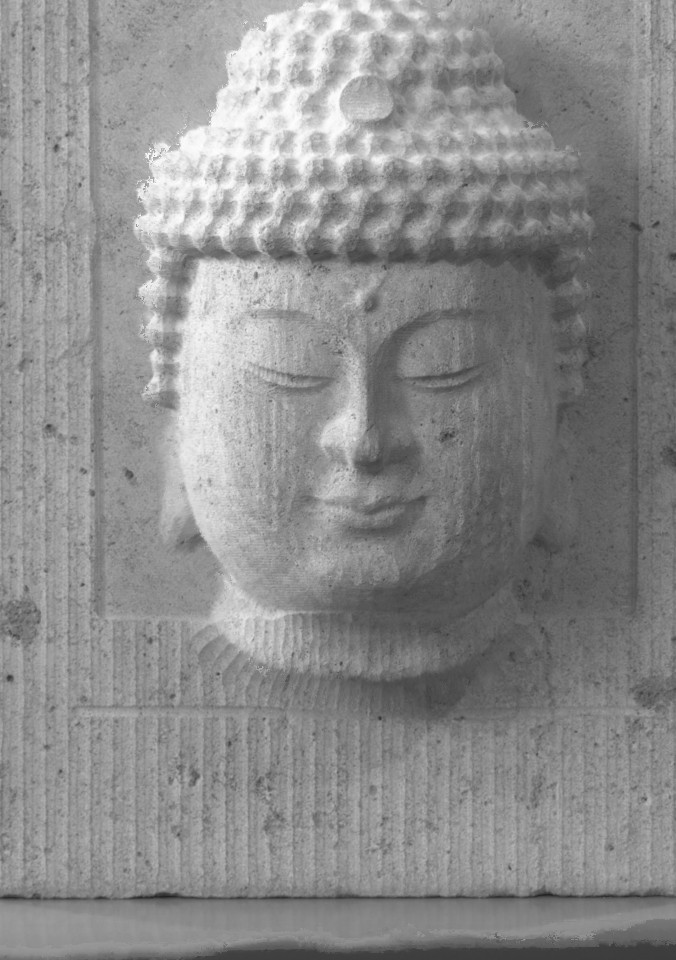
\includegraphics[width=55mm]{FIGS/Boudhas/Ort_IMG_5588.jpg}   &
   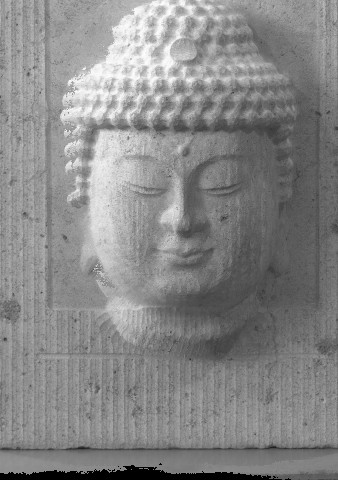
\includegraphics[width=55mm]{FIGS/Boudhas/Ort_IMG_5589.jpg}   &
   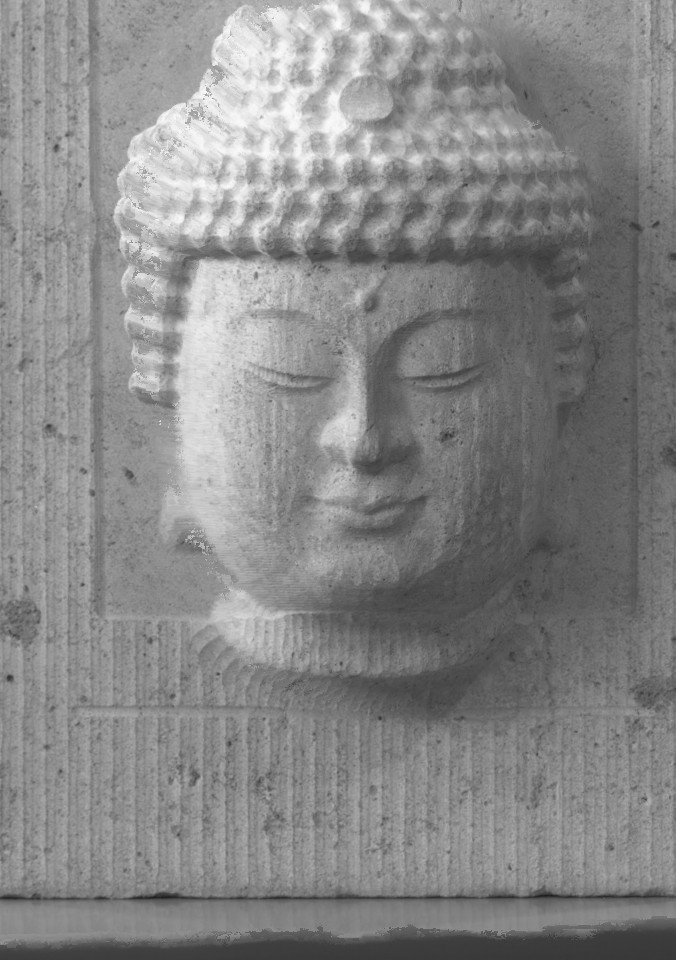
\includegraphics[width=55mm]{FIGS/Boudhas/Ort_IMG_5592.jpg}   \\ \hline  \hline
\end{tabular}
\label{Indiv:Ortho}
\caption{Three of the five individual ortho images}
\end{figure}



\begin{figure}
\begin{tabular}{||c|c||}
   \hline \hline
   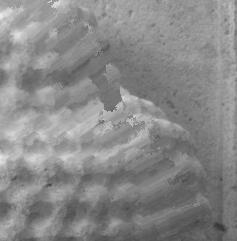
\includegraphics[width=80mm]{FIGS/Boudhas/PB-Ort_IMG_5591.jpg}   &
   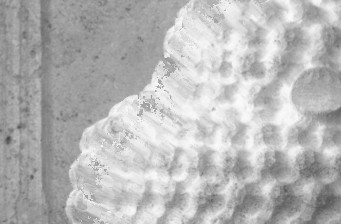
\includegraphics[width=80mm]{FIGS/Boudhas/PB-Ort_IMG_5592.jpg}   \\ \hline  \hline
\end{tabular}
\label{Pb:Indiv:Ortho}
\caption{Zoom on some problems of  individual ortho-image}
\end{figure}



\begin{figure}
\begin{tabular}{||c|c|c|c|c||}
   \hline \hline
   
\includegraphics[width=30mm]{FIGS/Boudhas/Incid_IMG_5588_8Bits.jpg} &
   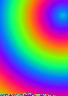
\includegraphics[width=30mm]{FIGS/Boudhas/Incid_IMG_5589_8Bits.jpg} &
   
\includegraphics[width=30mm]{FIGS/Boudhas/Incid_IMG_5590_8Bits.jpg} &
   
\includegraphics[width=30mm]{FIGS/Boudhas/Incid_IMG_5591_8Bits.jpg} &
   
\includegraphics[width=30mm]{FIGS/Boudhas/Incid_IMG_5592_8Bits.jpg} \\ \hline  \hline
\end{tabular}
\label{Incid:Ortho}
\caption{ Incidence images computed for ortho priority}
\end{figure}

In the exemple {\tt Param-Porto.xml}, the section specifying these inputs is:


{\scriptsize
\begin{verbatim}
    <SectionEntree>
           <FileMNT> ../MEC-7-Ter/Z_Num5_DeZoom1_LeChantier.xml </FileMNT>
           <KeySetIm>  NKS-Set-OfPattern@Ort_(.*)\.tif </KeySetIm>
           <KeyAssocMetaData > NKS-Assoc-ChangPrefixAndExt@Ort_@tif@PC_@xml  </KeyAssocMetaData>
           <KeyAssocNamePC >   NKS-Assoc-ChangPrefixAndExt@Ort_@tif@PC_@tif </KeyAssocNamePC>
           <KeyAssocNameIncH>  NKS-Assoc-ChangPrefixAndExt@Ort_@tif@Incid_@tif </KeyAssocNameIncH>
    </SectionEntree>
\end{verbatim}
}

The {\tt <FileMNT>} is an XML-meta-data file containing information about the DTM produced
by {\tt MicMac}. Its tags have been described in~\ref{Ex:GrTer:RA}. The ortho-mosaic produced
by {\tt Porto} will have the same geo-referencing as the DTM. The other arguments are
keys for describing sets and associations. The functioning is quite classical now:

\begin{itemize}
    \item {\tt <KeySetIm>} describes the set of individual ortho images;
    \item {\tt <KeyAssocMetaData>} is a key for computing the name of XML-Meta data from the name of individual ortho image;
    \item {\tt <KeyAssocNamePC>} is a key for computing the name of the \UNCLEAR{hidden part image} from the name of individual ortho image;
    \item {\tt <KeyAssocNameIncH>} is a key for computing the name of the incidence image from the name of individual ortho image;

    \item \UNCLEAR{this is the same key}, that is used with different parameters; this key allows to change the
          beginning (prefix) of a name and its extension.

\end{itemize}

Here is {\tt PC\_IMG\_5588.xml}, an example of one of the meta-data file:


{\scriptsize
\begin{verbatim}
<MetaDataPartiesCachees>
     <Done>true</Done>
     <Offset>0 0</Offset>
     <Sz>676 960</Sz>
     <Pas>1</Pas>
     <SeuilUse>3</SeuilUse>
     <SsResolIncH>10</SsResolIncH>
</MetaDataPartiesCachees>
\end{verbatim}
}

The important tags are:

\begin{itemize}
   \item {\tt <Offset>} and {\tt <Sz>} specify the position of the individual ortho-photo
         on the DTM. Because, of course, in real example, the individual ortho-photo  will be much smaller
         than the DTM or resulting mosaic, so it will be stored only a sub-rectangle of the global DTM;

   \item {\tt <SeuilUse>} is a real value, use \UNCLEAR{to threshold} the  images ({\tt PC\_IMG\_5588.tif} \dots) and
         defining which pixel must be used;

   \item {\tt <SsResolIncH>} is the resolution of incidence images ({\tt Incid\_IMG\_5588.tif} \dots)
         in fact as these images are very regular, it would be useless to store them at full resolution.
         
\end{itemize}


As this file have been generated automatically by {\tt MicMac}, in most cases you will
not need to modify it, but it is still good to understand a bit how things work,
in case of problems \dots


   % - - - - - - - -  -- -  - - - - - - - -  - - - - - - - - - - - - - - - - - - - - - - - -

\subsection{Output to Porto}

Once  all these inputs are \UNCLEAR{knowns}, %nom ou adjectif?
the mosaicing
algorithm is quite obvious:

\begin{itemize}
     \item for each pixel of  the ouput image:
     \begin{itemize}
          \item select the unmasked image having the lowest incidence.
     \end{itemize}
\end{itemize}

The parameters specifying the output are:

{\scriptsize
\begin{verbatim}
     <SectionSorties>
           <SzDalle>    1000            </SzDalle>
           <SzBrd>      100             </SzBrd>
           <NameOrtho>  Ortho-NonEg-Test-Redr.tif </NameOrtho>
           <NameLabels>  Label-Test-Redr.tif</NameLabels>
     </SectionSorties>
\end{verbatim}
}

{\tt NameOrtho} specifies the name of the ortho mosaic. {\tt NameLabels} is an optional
argument, when specified, {\tt Porto} creates a label image indicating for each pixel which 
individual  image is to be used for \UNCLEAR{filling the geometry}.  \UNCLEAR{Figure~\ref{Resul:Ortho}} %pas bon le nr de la fig
presents the main results.


\begin{figure}
\begin{tabular}{||c|c||}
   \hline \hline
   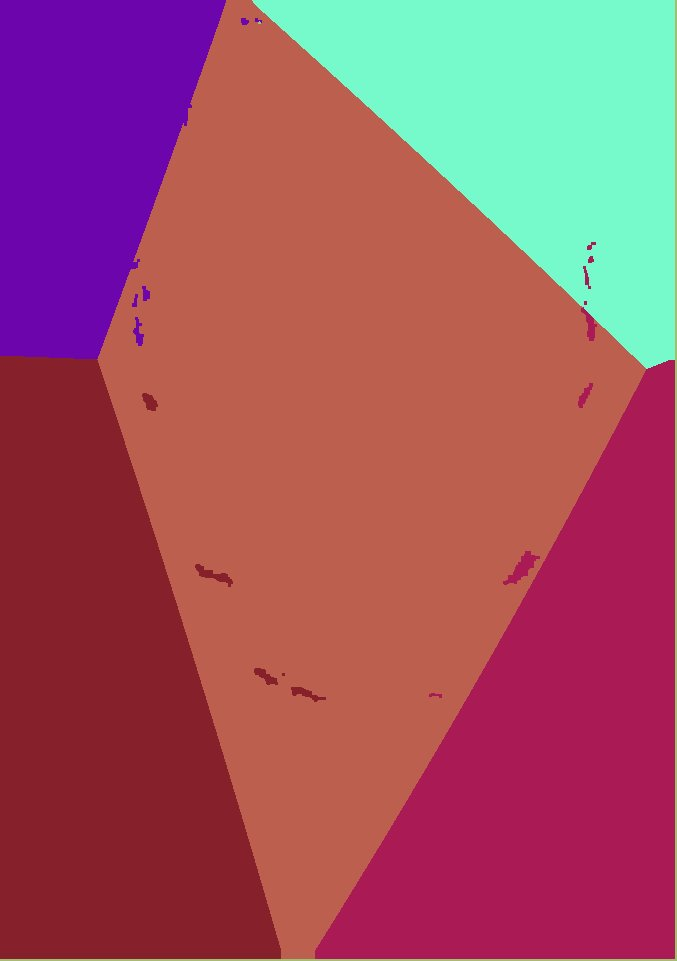
\includegraphics[width=80mm]{FIGS/Boudhas/Label-Test-Redr.jpg}   &
   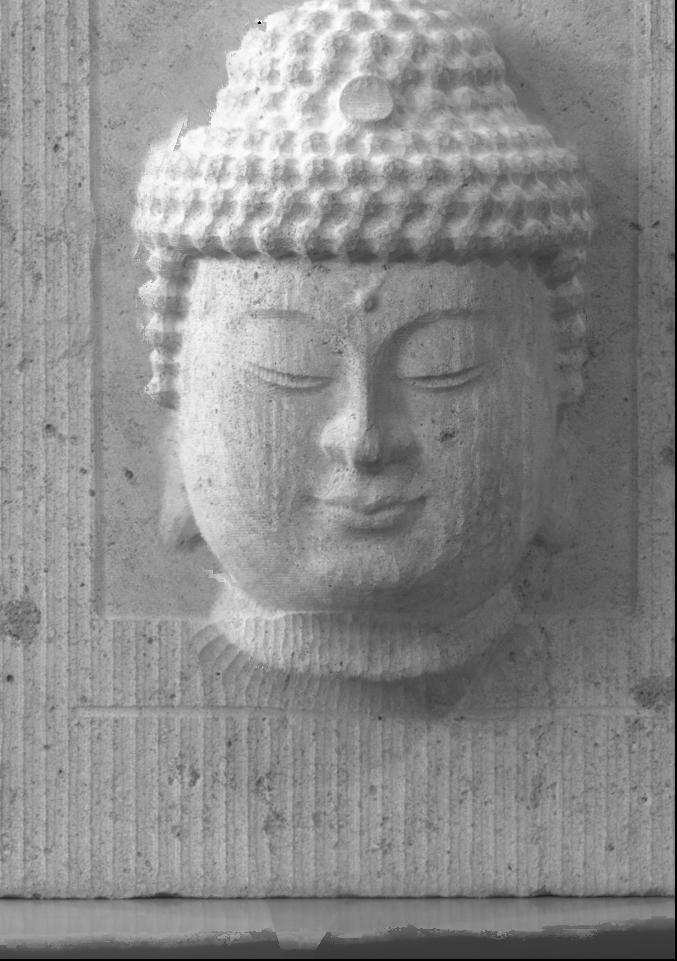
\includegraphics[width=80mm]{FIGS/Boudhas/Ortho-NonEg-Test-Redr.jpg}   \\ \hline  \hline
\end{tabular}
\label{Resul:Ortho}
\caption{Computed label images and resulting ortho images}
\end{figure}



   % - - - - - - - -  -- -  - - - - - - - -  - - - - - - - - - - - - - - - - - - - - - - - -
\subsection{Radiometric Equalization}





